% \begin{frame}
%   \begin{columns}
%     \begin{column}{0.5\textwidth}
%     \end{column}
%     \begin{column}{0.5\textwidth}
%     \end{column}
%   \end{columns}
% \end{frame}

\begin{frame}{Automate \texttt{ABC} sur FPGA : compléments}
  \begin{columns}
    \begin{column}{0.45\textwidth}
      \begin{itemize}
        \item Synthèse RTL/logique
        \begin{itemize}
          \item outil \texttt{Vivado Xilinx (AMD)}
        \end{itemize}
        \item Adaptation VHDL des interfaces :
        \begin{itemize}
          \item \texttt{switch} en va-et-vient : créé l'événement '\texttt{e}' d'entrée
          \item Affichage 7 segments : états '\texttt{s}' convertit en nibble.
        \end{itemize}
      \end{itemize}
    \end{column}
    \begin{column}{0.55\textwidth}
      \begin{center}
        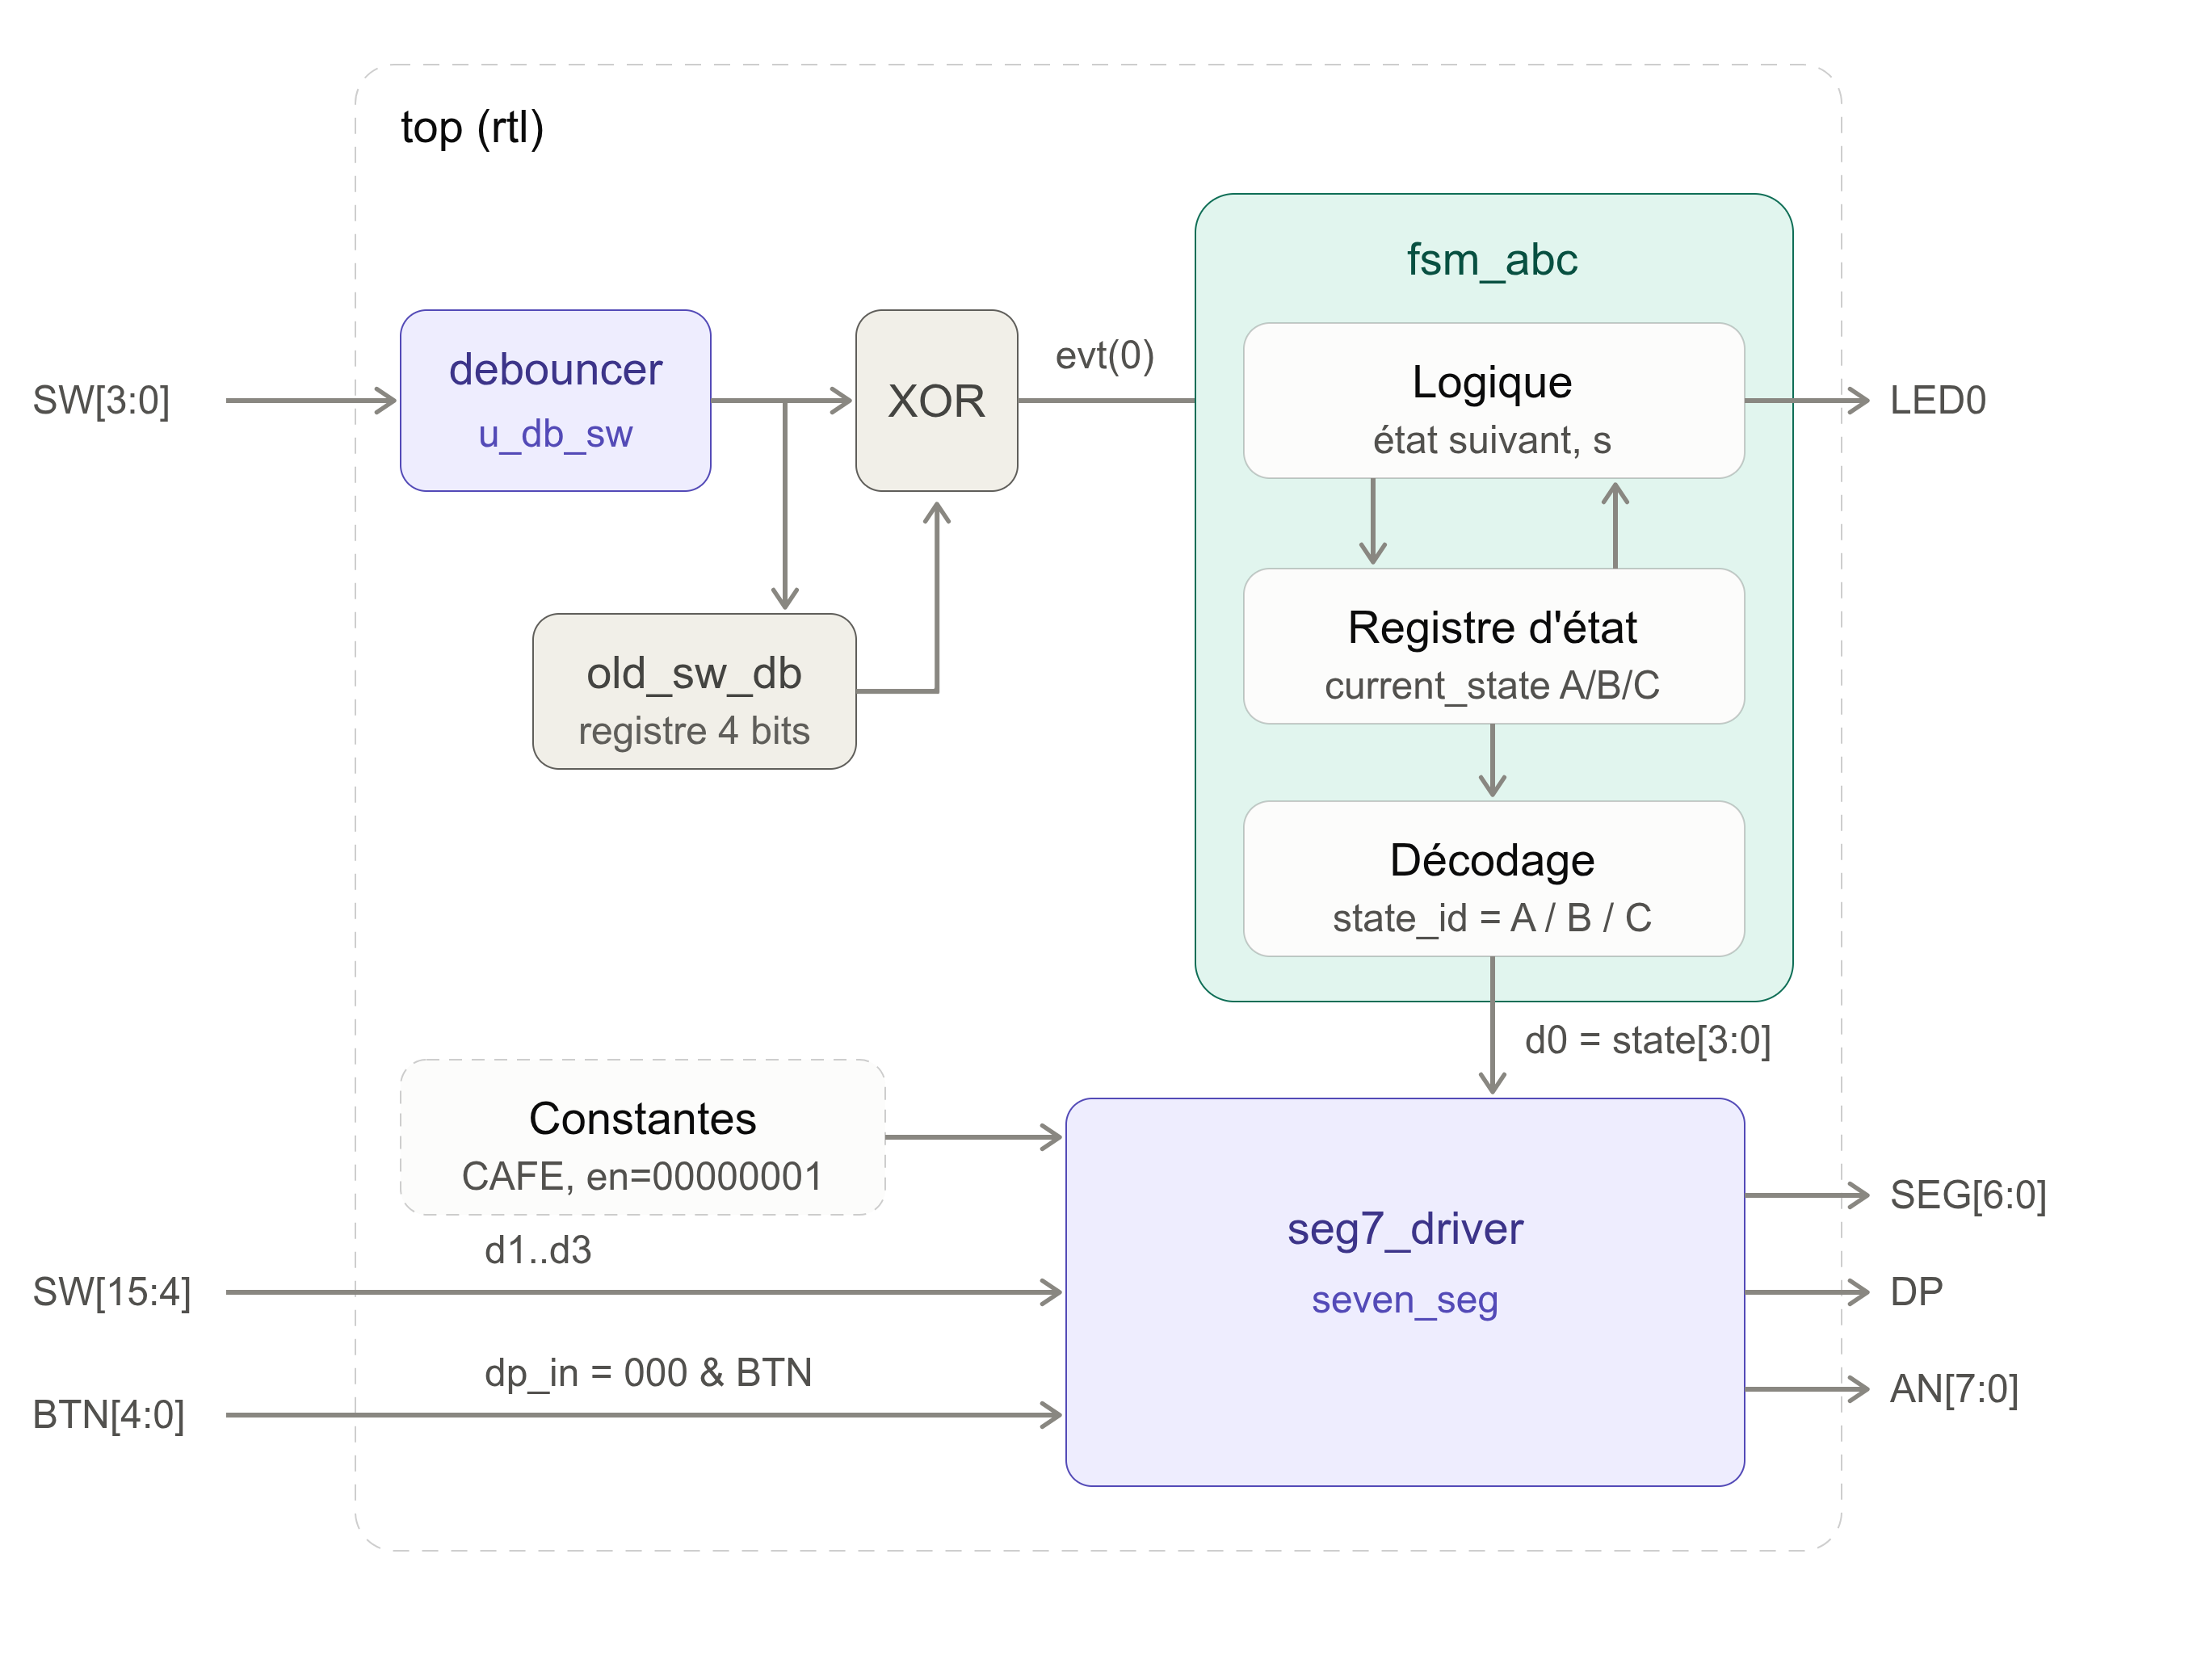
\includegraphics[scale=0.09]{./images/schematic_top_hierarchique.png}
      \end{center}
    \end{column}
  \end{columns}
\end{frame}

\begin{frame}{Composer des systèmes : exemple bi-processeur MIPS}
  Le jeu est désormais de \textbf{composer} des systèmes à partir de \textbf{composants}.
  \begin{itemize}
    \item De plus en plus gros.
    \item Approche récursive, constructive.
  \end{itemize}
  \begin{columns}
    \begin{column}{0.5\textwidth}
      \begin{center}
        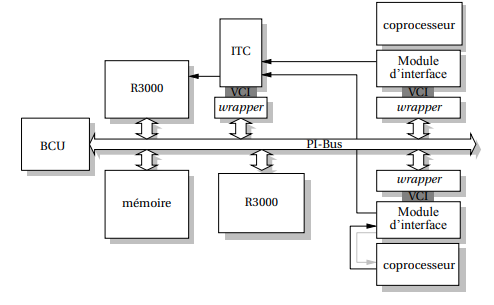
\includegraphics[scale=0.5]{./images/denis_hommais_arch_1.png}
      \end{center}
    \end{column}
    \begin{column}{0.5\textwidth}
      \begin{center}
        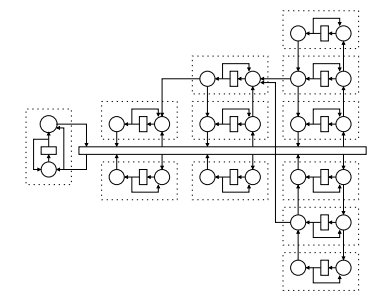
\includegraphics[scale=0.5]{./images/denis_hommais_arch_2.png}
      \end{center}
    \end{column}
  \end{columns}
\end{frame}
